%!TEX root = main.tex
\section{Introduction}
\label{sec:intro}
%
%\JW{Fixed: It would be nice to have a picture here showing how reaffirm is used -- ideally reaffirm would be a box that is detailed later on in section 3 ... but it would show the workflow for how a designer might use the tool.}
%
%\JW{Fixed: Somewhere in this motivation we need to assert that it is impossible to know all potential future attacks/vulnerabilities -- and this is where current techniques for secure-by-design systems engineering have shortcomings.}
%
A cyber-physical system (CPS) consists of computing devices communicating with one another and interacting with the physical world via sensors and actuators. Increasingly, such systems are everywhere, from smart buildings to autonomous vehicles to mission-critical military systems. 
%
The rapidly expanding field of CPSs precipitated a corresponding growth in security concerns for these systems. The increasing amount of software, communication channels, sensors and actuators embedded in modern CPSs make them likely to be more vulnerable to both cyber-based and physics-based attacks~\cite{wan2015security, wasicek2014aspect, kocher2004security, al2015design, gamage2010enforcing}. As an example, \emph{sensor spoofing} attacks to CPSs become prominent, where a hacker can arbitrarily manipulate the sensor measurements to compromise secure information or to drive the system toward unsafe behaviors. Such attacks have successfully disputed the braking function of the anti-lock braking systems~\cite{Shoukry2013,al2015design}, and compromised the insulin delivery service of a diabetes therapy system~\cite{li2011hijacking}. Alternatively, attackers can gain access to communication channels to either manipulate the switching behavior of a smart power grid~\cite{liu2011class} or disable the brake system of a modern vehicle~\cite{koscher2010experimental}. Generally, constructing a behavioral model at design time that offers resiliency for all kinds of attacks and failures is notoriously difficult. 
% \JW{Fixed: do you mean physics-based attacks? physical-based attacks doesn't make sense grammatically.}
%Therefore, it is essential for a designer to build a CPS model with a resilient capability to cope with different attack scenarios. However, constructing a behavioral model at design time that offers resiliency for all kinds of attacks and failures is notoriously difficult as a) it requires investigating many sub-components in an integrated manner, especially for a large-scale CPS, and b) it is impossible to know all potential future attacks and vulnerabilities.
%
%Current techniques for secure-by-design systems engineering do not provide a formal way for a designer to specify a resiliency pattern to automatically repair system models based on evolving resiliency requirements under unanticipated attacks. %The goal of the proposed methodology in this paper is to  

%Our vision of \toolreaffirm is that a designer can incorporate the toolkit as an efficient repair mechanism in the model-based design paradigm to iteratively improve the original design for resiliency when new vulnerabilities are identified and requirements evolve.
%The goal of the proposed methodology and the associated toolkit, which we call REAFFIRM, is to facilitate integration of evolving cyber-physical resiliency requirements in the model-based design of CPSs. 
%However, many CPSs are developed today without considering resiliency at all. Model-based system developers often neglect or incompletely consider incorporating resiliency patterns in their designs. 
%\JW{Fixed: Again, this is a strong statement -- we might want to play nicer with the reviewers and change the wordings.  It isn't that designers don't consider resiliency requirements -- there just isn't a formal way to analyze and repair system models based on evolving resiliency requirements.}
%
%
% 
%Toward addressing this problem, we offer an effective way for model-based system developers to specify and incorporate resiliency patterns in their designs. Our approach allows a designer to write a simple model transformation script described a potential edit for an original model to provide resilience when vulnerabilities are discovered.
%
%Then the model transformation tool of \toolreaffirm will take the transformation script and the original model as inputs and generate a candidate resilient model that contains parameters whose values will be determined by the model synthesizer of \toolreaffirm. As a result, \toolreaffirm outputs a completed model which satisfies a given safety property formally specified as a Signal Temporal Logic (STL)~\cite{maler2004monitoring} formula. 
%
%Our vision of \toolreaffirm is that a designer can incorporate the toolkit as an efficient repair mechanism in the model-based design paradigm to iteratively improve the original design for resiliency when new vulnerabilities are identified and requirements evolve.   


%
%A general solution would be to formally specify safety properties of a CPS that protect the system against possible adversarial attacks using formalisms such as signal temporal logic (STL)~\cite{maler2004monitoring} and to then iteratively improve the design using \emph{falsification}~\cite{nghiem2010monte}, which would automatically identify vulnerabilities in the design. 

%Model-based design offers a promising approach for assisting developers to build a reliable and secured CPSs in a systematic manner~\cite{alur2015principles,lee2000s,barthe2004secure}. 
%
\begin{figure}[t!]%
	\centering%
    %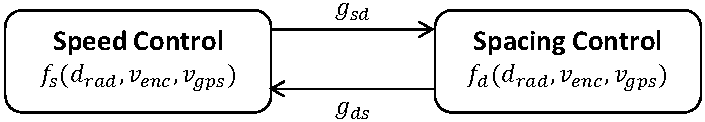
\includegraphics[width=0.48\textwidth]{image/acc_abstract_model}%
		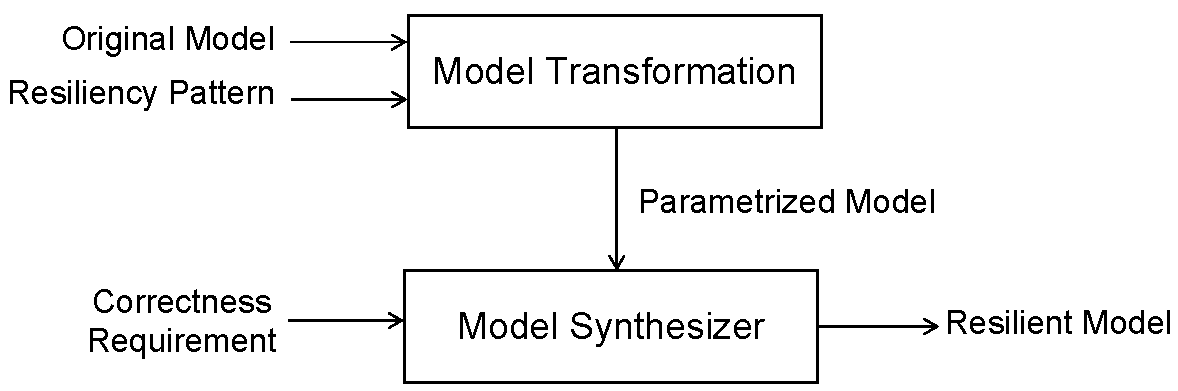
\includegraphics[width=0.48\textwidth]{image/overview}%
		%\includegraphics[trim = 17mm 85mm 17mm 0mm, clip, width=0.95\textwidth]{image/spectral_signal}%
		%\vspace{-1em}
	\caption{\toolreaffirm Overview.}%
	\figlabel{overview}%
	%\vspace{-1em}
\end{figure}%
Traditionally a model of a CPS consists of block diagrams describing the system architecture and a combination of state machines and differential equations describing the system dynamics~\cite{alur1995algorithmic}. Suppose the designer has initially constructed a model of a CPS that satisfies correctness requirements, but at a later stage, this correctness guarantee is invalidated, possibly due adversarial attacks on sensors, or violation of environment assumptions. Current techniques for secure-by-design systems engineering do not provide a formal way for a designer to specify a resiliency pattern to automatically repair system models based on evolving resiliency requirements under unanticipated attacks. 

In this paper, we propose a new methodology and an associated toolkit, which we call \toolreaffirm, to assist a designer in repairing the original behavior model to generate the completed behavior model with resilience. %\JW{Fixed: We haven't introduced the notion of a partial model yet -- this will be confusing to the reviewers.}
%
The proposed technique relies on designing a collection of \emph{potential edits} (or \emph{resiliency patterns}) to the original model to generate the new model whose parameters values can be determined by solving the \emph{parameter synthesis problem}. 
%\JW{Fixed: does designing a collection of resiliency patterns solve the model synthesis problem?  I don't think it does -- perhaps we can re-word this.}
%
%\JW{Fixed: This seems trivial -- why do we need a tool to do this?  Perhaps you can change "conservative" to "trivial" -- and move this sentence to after the next sentence.}
%
%
\figref{overview} shows an overview of \toolreaffirm, which contains two mains modules including a \emph{model transformation} and a \emph{model synthesizer} built on top of the falsification tool Breach~\cite{donze2010breach}.
\toolreaffirm takes the inputs including the original system modeled as a Simulink/Stateflow (SLSF) diagram, the resiliency pattern specified by the designer and the safety requirement expressed as a Signal Temporal Logic (STL)~\cite{maler2004monitoring} formula, and then utilizes the falsification tool Breach to synthesize the repaired SLSF model that satisfies the safety requirement.

%There is currently lack of an automated mechanism that can efficiently repair the initial design and provide resilience.  
%
%
%Many significant research have been introduced to build resilient CPSs such as the approach proposed in~\cite{fitzgerald2012rigorous} that can be used to design a resilient CPS through co-simulation of discrete-event models, a modeling and simulation integration platform for secure and resilient CPS based on attacker-defender games proposed in~\cite{koutsoukos2018sure} with the corresponding testbed introduced in~\cite{neema2018integrated}, and the resilience profiling of CPSs presented in~\cite{jackson28resilience}. Although these approaches can leverage the modeling and testing for a resilient CPS, they do not offer a model repair mechanism as well as a generic approach to design a resiliency pattern when vulnerabilities are discovered. In most of the case, a designer needs to rebuild the system from scratch, which requires a lot of time and efforts.
%
%
 %Moreover, there is a lack of a generic method for a designer to specify a resiliency pattern.  
%
 %
%
%

%Suppose the designer has initially constructed a model of a CPS that satisfies correctness requirements, but at a later stage, this correctness guarantee is invalidated, possibly due to the emergence of new requirements, or adversarial attacks on sensors, or violation of environment assumptions. 
%
%

 %For example, a trivial way ensuring safety upon encountering an unexpected or hazardous situation is to hand over control to a baseline safety controller. 
%
%\OS{Fixed: "known" may not be the right word.  Maybe "specified by the designer."}  
%
%The resilient version generated by \toolreaffirm may have additional modes of operation as well as new transitions between different modes, and as a result, has resilient behaviors.
%

%The designer can construct a resiliency pattern to repair the original model based on the feedback derived from a counterexample generated by the \emph{falsification} tool embedded within \toolreaffirm. 
%%
%%\OS{Fixed: I don't quite understand the message of this sentence.  Are behaviors resilient because they are derived from a counterexample?  They are not added due to the counterexample.  On the contrary, counterexamples remove some behaviors added by the pattern because they do not fix the problem.}
%%
%Since a counterexample characterizes undesirable, or \emph{shall not},\OS{This is language specific to CASE.  Not everyone will understand.} situations, it can naturally describe how a system should respond when a particular sensor fails, or a previously unanticipated attack is identified. The model synthesizer within \toolreaffirm can automatically integrate such a counterexample with state-machine based models thus allowing an incremental design to support resiliency.
%
%
To allow the designer to specify resiliency patterns we have developed a new \emph{model transformation language} for hybrid systems, called HATL.
%
A HATL script is a sequence of statements that describe the modifications over the structure of hybrid systems molded as hybrid automata~\cite{alur1995algorithmic}.  An example of such a modification is adding new modes of operation as well as new transitions between different modes into the initial model to create the new one. 
%
The proposed language allows a designer to specify a resiliency pattern in a generic manner, programmatically modify the initial design without knowing the internal structures of a system. The interpreter of HATL is implemented in Python with the backend is extensible for the translations to different modeling frameworks of hybrid systems. The current implementation of HATL supports the translation of a HATL script to an equivalent MATLAB script that can perform the model transformation for Stateflow models.
%
To the best of our knowledge, this transformation language is the first effort to design a programmable pattern to repair CPSs models for improving resiliency.
%
%\OS{Fixed: I would rephrase this to make the connection with the earlier statement that a pattern needs to be specified as input. Consider "to allow the designer to specify a resilience pattern, we have developed..."}
%For example, a conservative way ensuring safety upon encountering an unexpected or hazardous situation is to hand over control to a baseline safety controller.

For evaluation, we apply \toolreaffirm to automatically synthesize the repaired models for two proof-of-concept case studies in the domains of automotive control and smart power systems. The first case study is a simplified model of an adaptive cruise control (ACC) system under the GPS sensor spoofing attacks, and the resiliency pattern to fix the model is to use the wheel encoders, which are additional (redundant) sensors for estimating a vehicle's velocity. The second case study is a single-machine infinite-bus model (SMIB), which is an approximation of a smart power grid, under a sliding-mode attack. In this case, the mitigation strategy is to increase the minimal dwell-time to avoid rapid changes between different operation modes. 
%
%
%
Overall, the main contributions of the paper are summarized as follows.
%
\begin{enumerate}[leftmargin= 2 em]
\item the methodology to facilitate the model-based repair for improving the resiliency of CPSs against unanticipated attacks and failures,
\item the design and implementation of an extensible model transformation language for specifying resiliency patterns used to repair CPS models,
\item the end-to-end design and implementation of the toolkit, which integrates the model transformation and the model synthesis tools to automatically repair CPS models,
\item the applicability of our approach on two proof-of-concept case studies where the resilient CPS models can be automatically constructed to mitigate practical attacks.
\end{enumerate}
%\JW{Fxied: an extensible?}
%
%We anticipate that our methodology proposed along with \toolreaffirm for automatically conducting the model repair and specifying the patterns of resiliency will be contributions of significant interest to the research community in the design of resilient CPSs. Our vision of \toolreaffirm is that a designer can incorporate the toolkit as an efficient repair mechanism in the model-based design paradigm to iteratively improve the original design for resiliency when new vulnerabilities are identified and requirements evolve.
%
%

The remainder of the paper is organized as follows.~\secref{overview} presents an overview of our proposed methodology through a simplified example of an adaptive cruise control (ACC) system, and introduces the architecture of \toolreaffirm.~\secref{transformation} describes our model transformation language used to design a resiliency pattern for hybrid systems.~\secref{synthesis} presents the model synthesizer of \toolreaffirm.~\secref{result} presents two proof-of-concept case studies that illustrate the capability of \toolreaffirm in automatically repairing the original models of a) the ACC system under GPS sensor spoofing attacks and b) the smart power grid system under a sliding-mode attack.~\secref{rw} reviews the related works to \toolreaffirm.~\secref{conclude} concludes the paper and presents future research directions for the proposed work.
% \JW{Fixed a toy example ... no need to say "running" -- that will be obvious.}





